\section{Durchführung}
Der Versuch wird nach Abbildung \ref{fig:aufbau} aufgebaut.
\begin{figure}
    \centering
    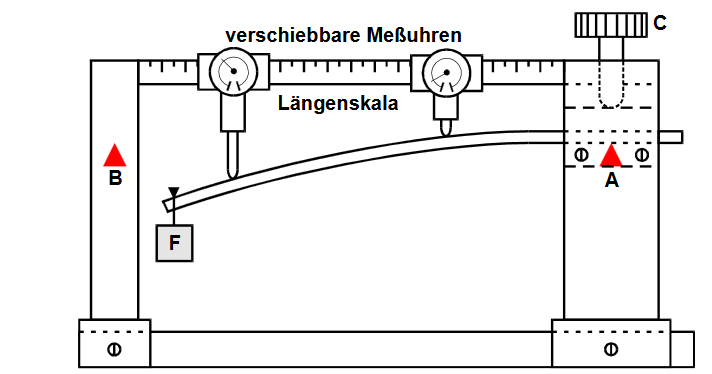
\includegraphics[width=\textwidth]{content/aufbau.png}
    \caption{Versuchsaufbau}
    \label{fig:aufbau}
\end{figure}
Der zu untersuchende Stab kann entweder in C eingespannt werden oder zwischen A und B aufgehängt werden.
Die Auslenkung geschieht über ein Gewicht, welches entweder am Stabende oder der Stabmitte angehangen wird.
Dabei wird das Gewicht so gewählt, dass die Auslenkung sich zwischen $3-7\si{\milli\meter}$ befindet.
Diese lässt sich mit Messuhren bestimmen, welche auf der $x$-Achse beweglich sind.
In $\SI{2}{\centi\meter}$ Abständen wird die Auslenkung gemessen.
Es ist nicht davon auszugehen, dass die Stäbe exakt gerade sind.
Deshalb muss die Messung für jeden Abstand $x$ jeweils mit als auch ohne Last durchgeführt werden.
Die tatsächliche Auslenkung ergibt sich dann aus der Differenz der beiden Werte.
Die rechte Seite der Gleichung wird mit $-1$ multipliziert, da die Messuhren Auslenkungen nach oben messen.
\begin{equation}
  D(x)=D_0(x) - D_M(x)
\end{equation}
Nach der Messung wird der Stab vermessen und gewogen.
